\section{Study Design and Tests}
\label{sec:methods}

We define \emph{educational personality} operationally as recurring defaults
and conditional response patterns that help predict a deployment's behavior on
new educational inputs. The unit is a deployment configuration, including the
requested and returned model names, provider, observation period, and generation
settings. We study MiniMax-M3, MiniMax-M2.7, GLM-5.3, DeepSeek-V4-Pro, and
Doubao-Seed-2.0-Lite. This definition neither assumes human traits nor requires
an invariant ranking across contexts. Figure~\ref{fig:study-design} shows how
the design connects recurrence, prediction, and prompt effects. Complete
materials, measurement rules, estimation details, and protocol history appear
in Appendix~\ref{app:detailed-methods}.

\begin{figure}[t]
\centering
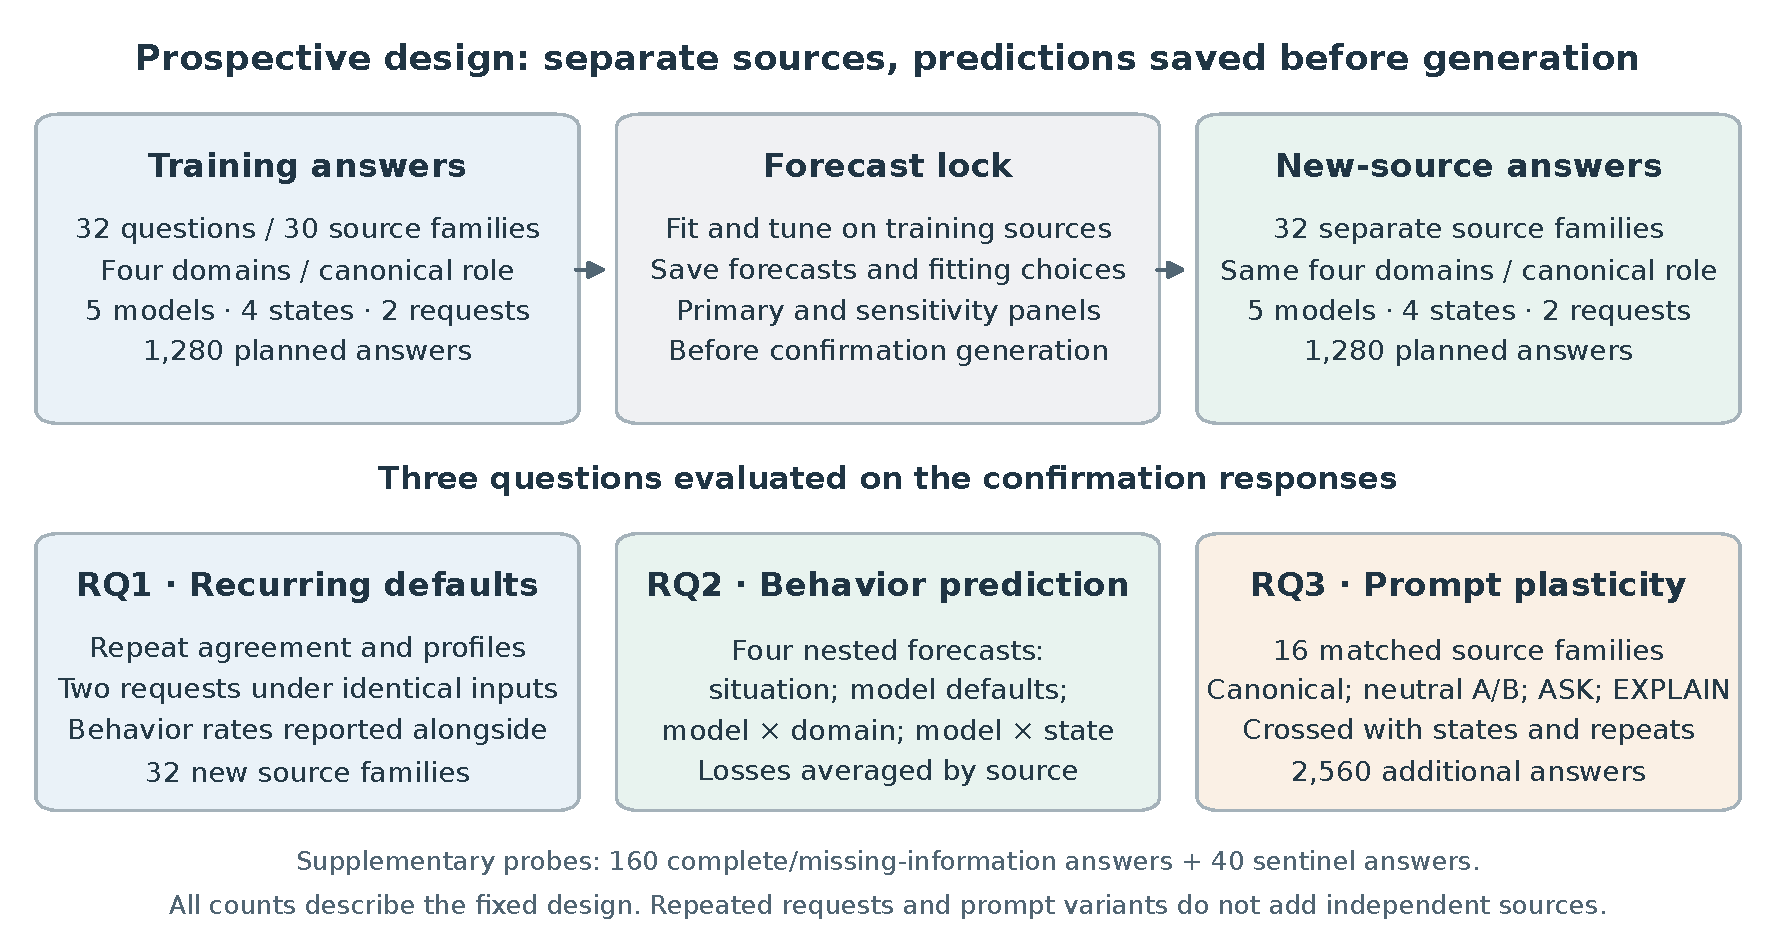
\includegraphics[width=\linewidth]{figures/study_design.pdf}
\caption{Prospective design, with realized response counts. Each main question
crosses five configurations, four student-work/affect conditions, and two
requests. Main training and confirmation source families are separate.
RQ1 and RQ2 use the 32 canonical confirmation sources; RQ3 reuses 16 of them
under additional role arms. Repetitions and prompt variants do not add
independent sources. The four nested forecasts are accompanied by the
training-only style competitor and the sensitivity analyses described below.}
\label{fig:study-design}
\end{figure}

\subsection{Exploration, Measurement Development, and Confirmation}

The million-record archive informed exploration. Its 899,025 successful,
variant-preserving deduplicated records span different roles; 68,799 belong to
nine tutor-response settings under the current-adapter role audit. Historical
prompt and deployment provenance is incomplete (Appendix~A). We therefore keep
archive findings separate from the prospective experiment. An excluded pilot
of 160 answers develops the event measures reported in
Section~\ref{sec:measurement-development}.

The prospective experiment contains 32 training questions in 30 conservative
source families and 32 confirmation questions in 32 separate families. Each
partition has eight questions in mathematics, science, language, and logic/data
reasoning. Related training questions remain grouped during validation, and the
four pilot templates and their numerical substitutions are excluded. Research
agents authored the problems and student messages; two model reviewers checked
all 64 question packages before freezing. The confirmation target is new
sources within these four domains, not unseen domains or representative
classroom interactions.

Each question crosses an erroneous attempt versus correct unfinished work with
an explicitly calm versus frustrated student statement. The work contrast
bundles correctness and progress; the affect contrast manipulates a textual
cue. Every main condition supplies the same instructor reference solution,
marked as unseen by the student. This equalizes solution availability without
eliminating ability or instruction-following differences. Each model--input cell
receives two requests at temperature 0.7 and an 8,192-token output budget.
Training and canonical confirmation each contain 1,280 responses. Additional
prompt arms contribute 2,560 responses on 16 confirmation sources. Secondary
information-opportunity probes and cross-stage sentinels add 160 and 40
responses, respectively, for 5,320 tutor generations. These repetitions
and variants do not add independent sources.

\subsection{Observable Behavior and Recurrence (RQ1)}

The three pilot-selected primary events are \emph{answer revelation}, an
explicit final resolution regardless of correctness; \emph{reasoning
elicitation}, an invitation for the student to perform reasoning that the tutor
has not immediately answered; and \emph{affect acknowledgement}, explicit
recognition of feeling or difficulty beyond generic praise or politeness. These
co-occurring actions are endpoints, not independent latent factors. Five
secondary events remain reported regardless of their results.

MiniMax-M3, DeepSeek-V4-Pro, and GLM-5.3 each code every visible response using
student context, the reference target, and original answer lines. Generator
identity, role arm, repetition, and partition labels are withheld; output style
may still reveal identity. Positive codes require existing nonempty evidence
lines. Primary labels use the majority of three structurally valid codes;
traceability and agreement do not establish semantic ground truth. Repairs
address completion or structure failures, never event labels or disagreement.
One missing training code required a disclosed larger-budget amendment before
prediction locking. Six missing confirmation codes later required a separately
recorded amendment after the original repair limit. Appendix~\ref{app:detailed-methods}
preserves their scope and failures; a supplemental missing-code sensitivity
checks whether the primary conclusions depend on the amended measurements.

RQ1 reports model event rates, state-specific profiles, and positive, negative,
and total agreement across the two requests, with source clustering. Constant
behavior can yield perfect agreement, so recurrence is interpreted alongside
prevalence and predictive value.

\subsection{Locked Prediction on New Sources (RQ2)}

For each event, four nested logistic predictors successively include
subject-by-student-state context, model identity, model-by-subject interactions,
and model-by-student-state interactions. Training-only orthogonalization and
standardization preserve the ridge geometry of earlier feature blocks.
Source-grouped training validation selects the penalty from
$\{0.1,1,10,100\}$; the intercept is unpenalized. All fitted parameters, tuning
choices, and confirmation probabilities are locked before any confirmation
tutor response is generated. No confirmation answer or label enters prediction
fitting. A descriptive style competitor uses only training profiles of log word
count and marked-line fraction.

For each primary event, we test two Brier-loss improvements: adding model
defaults to context, and adding student-state interactions to the
model-by-subject predictor. Losses are averaged within source and equally
across 32 confirmation sources. Six one-sided paired source-level tests use
Holm correction; absolute losses, all gain signs, and source-bootstrap intervals
are reported. Intervals condition on the fitted training profiles and a
source-sampling approximation, not uncertainty over all educational settings
or model families.

\subsection{Prompt Effects and Alternative Explanations (RQ3)}

On 16 sources selected by a frozen hash, each model receives every student state
under the canonical role, two neutral role paraphrases, and explicit ASK and
EXPLAIN instructions. Paired source-level event-rate differences measure both
average displacement and model/state heterogeneity. The neutral equivalence
reference is $\pm0.10$. Nominal multiplicity-adjusted paired-$t$ intervals are
retained, but the additional bounded-source check is too imprecise at sixteen
sources to establish population equivalence. Nonsignificance does not establish
stability. ASK/EXPLAIN effects quantify instruction-driven behavior, not better
teaching. Joint revelation/elicitation rates allow both actions to co-occur
without inferring their order.

Pre-confirmation sensitivity specifications include eight coding panels, five
leave-one-generator analyses, and 200 training-source resamples. Mathematics
and content-error screens evaluate the locked forecasts without refitting;
flagged answers remove the complete five-model comparison slot. Two content
reviewers also receive twelve agent-authored diagnostic controls. These checks
assess dependence on measurement, configurations, training material, and errors;
they do not establish human ground truth or causal control of ability. Their
precise timing, retained coverage rules, and interpretation limits are given in
Appendix~\ref{app:detailed-methods}.
